\section{Résultats}\label{Sect_Resultats}
	Cette section présente les résultats des différents modèles testés pour chacune des bases de données. En premier lieu, une analyse graphique des raccordements de lois est faite pour avoir un aperçu de l'adéquation de chaque modèle. En deuxième lieu, un calcul statistique de l'adéquation des lois de sévérité est présenté pour comparer les modèles de façon plus formel. En troisième lieu, des modèles agrégés sont proposés pour finalement calculer les mesures de risque $VaR$ et $TVaR$.
 
 \subsection{Résultats - Analyse graphique}
 
	\subsubsection{\texttt{norwegianfire}}
	En commençant avec la base de données \texttt{norwegianfire}, on présente pour chacune des lois testées les graphiques quantiles-à-quantiles sur le support des petites valeurs et des grandes valeurs.
		
		\paragraph{Loi composite lognormale - Pareto:} Avec la continuité et la dérivabilité au point $\theta$, les estimateurs des paramètres sont $\hat{\theta} = 1\,288$, $\hat{\alpha} = 1,2987$ et $\hat{\sigma}=0,82812$.
		
		\begin{figure}[H]
			\begin{center}
				\begin{subfigure}[b]{0.45\textwidth}
					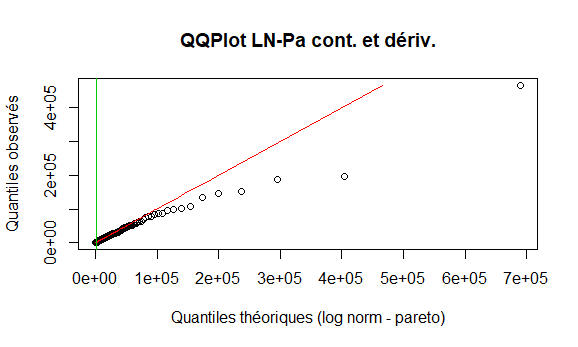
\includegraphics[scale=0.54]{Graphiques/QQ_LN_Pa_cont_dev} 
					\caption{Quantiles sur le support complet.} \label{QQplot_LN_Pa_conde}
				\end{subfigure}
				\begin{subfigure}[b]{0.40\textwidth}
					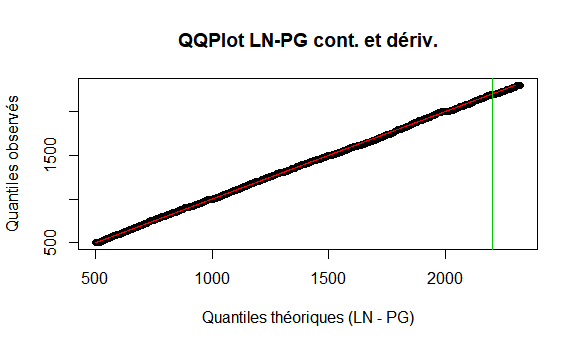
\includegraphics[scale=0.54]{Graphiques/QQ_LN_PA_contdiv_t1} 
					\caption{Quantiles de la lognormale pour $x<\theta$.} \label{QQplot_LN_Pa_conde_2}
				\end{subfigure}
				\renewcommand{\figurename}{Illustration}
				\caption{\textit{QQplots} - \texttt{norwegianfire} - LN-Pareto.}
			\end{center}
		\end{figure}
	
		Dans l'illustration \ref{QQplot_LN_Pa_conde}, on observe une bonne adéquation pour les valeurs en dessous de $100\,000$ \footnote{Rappel: Les montants affichés sont en excédent de $500\,000$ couronnes norvégiennes.}. Cependant, pour les données supérieures à ce montant, on trouve que le modèle n'est pas adéquat.  On remarque aussi que le seuil ($\theta$) estimé est relativement petit. La portion lognormale ne comprends que $61\%$ des données ($\hat{F}_n(\theta) = 0,613$, où $\hat{F}_n(\theta)$ est la fonction de répartition empirique). \\
		
		Lorsque l'on considère l'approche avec $\theta$ fixé, on observe un changement de comportement entre les valeurs de $20\,000$ et de $30\,000$ dans la fonction d'excès moyen présenté dans l'illustration \ref{Graph_Norwegianfire_MeanExcess}. On fixe $\theta = 22\,669$ (qui est le $9\,100$-ème statistique d'ordre) et on estime $\hat{\mu} =4,834\,589$, $\hat{\sigma}=1,624\,245$ et $\hat{\alpha} = 1,540\,549$.
		
		\begin{figure}[H]
			\begin{center}
				\begin{subfigure}[b]{0.45\textwidth}
					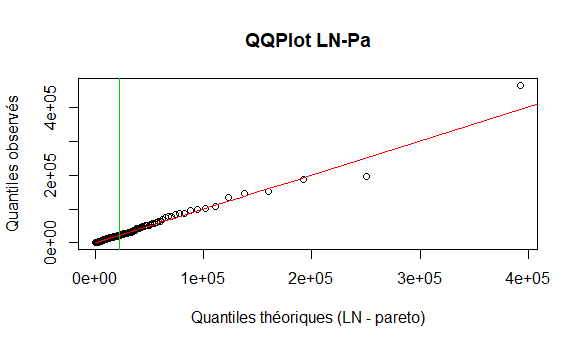
\includegraphics[scale=0.54]{Graphiques/QQ_LN_PA_choix} 
					\caption{Quantiles sur le support complet.} \label{QQplot_LN_Pa_choix}
				\end{subfigure}
				\begin{subfigure}[b]{0.4\textwidth}
					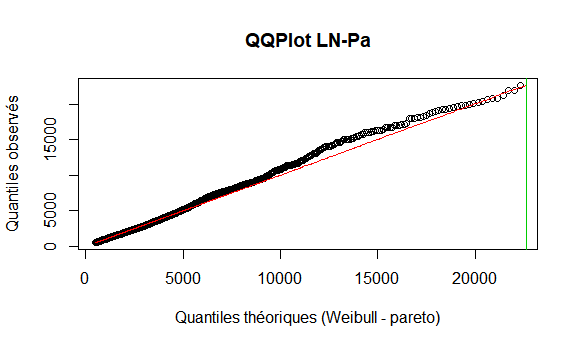
\includegraphics[scale=0.54]{Graphiques/QQ_LN_PA_choix_t1} 
					\caption{Quantiles de la lognormale pour $x<\theta$.} \label{QQplot_LN_Pa_choix_2}
				\end{subfigure}
				\renewcommand{\figurename}{Illustration}
				\caption{\textit{QQplots} - \texttt{norwegianfire} - LN-Pareto - $\theta$ fixé.}
			\end{center}
		\end{figure}
	
		De l'illustration \ref{QQplot_LN_Pa_choix_2}, on observe que l'adéquation pour la partie lognormale est un peu moins bonne que pour le modèle respectant la continuité et la dérivabilité. Cependant, pour les valeurs élevées, on surestime moins les montants de sinistres. L'ajustement est donc meilleur. Par contre, comme la densité présente un saut au point $\theta$, elle n'est pas continue et dérivable à ce point. 
		
		\paragraph{Loi composite lognormale et Pareto généralisée:} Avec la continuité et la dérivabilité au point $\theta$, on estime les paramètres et on obtient $\hat{\theta} =2\,204,333\,480$, $\hat{\lambda}=-20,958\,168$, $\hat{\alpha} =1,320\,166$ et $\hat{\sigma}= 1,143\,788$.
	
		\begin{figure}[H]
			\begin{center}
				\begin{subfigure}[b]{0.45\textwidth}
					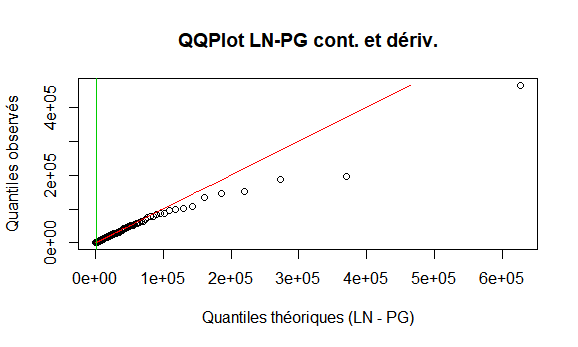
\includegraphics[scale=0.54]{Graphiques/QQ_LN_PG_condev} 
					\caption{Quantiles sur le support complet.} \label{QQplot_LN_PG_conde}
				\end{subfigure}
				\begin{subfigure}[b]{0.4\textwidth}
					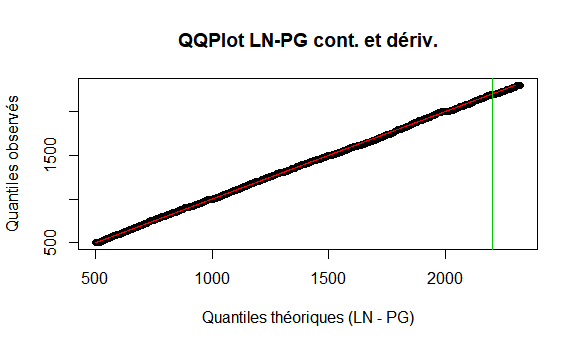
\includegraphics[scale=0.54]{Graphiques/QQ_LN_PA_contdiv_t1} 
					\caption{Quantiles de la lognormale pour $x<\theta$.} \label{QQplot_LN_PG_conde_2}
				\end{subfigure}
				\renewcommand{\figurename}{Illustration}
				\caption{\textit{QQplots} - \texttt{norwegianfire} - LN-PG.}
			\end{center}
		\end{figure}
		
		L'illustration \ref{QQplot_LN_PG_conde} montre un comportement similaire au modèle composite lognormal - Pareto simple. Toutefois, la portion lognormale comprends $81\%$ des données; ce qui est plus élevé que lorsque la deuxième loi du raccordement est une Pareto de type 1. En ignorant la continuité et la dérivabilité, on fixe $\theta = 22\,669$ et on trouve $\hat{\mu} = 4,834\,589$, $\hat{\sigma}=1,624\,245$, $\hat{\lambda} =  4\,604,525\,53$ et $\hat{\alpha} = 1,728\,66$.
		
		\begin{figure}[H]
			\begin{center}
				\begin{subfigure}[b]{0.45\textwidth}
					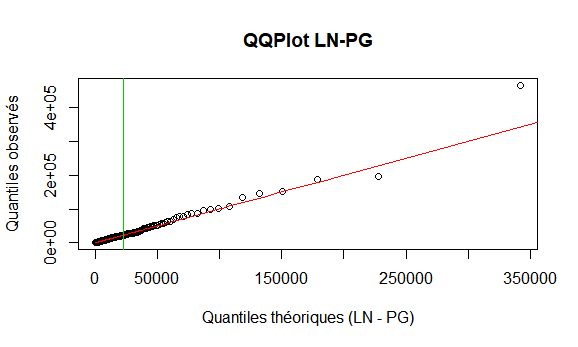
\includegraphics[scale=0.54]{Graphiques/QQ_LN_PG_choix} 
					\caption{Quantiles sur le support complet.} \label{QQplot_LN_PG_choix}
				\end{subfigure}
				\begin{subfigure}[b]{0.4\textwidth}
					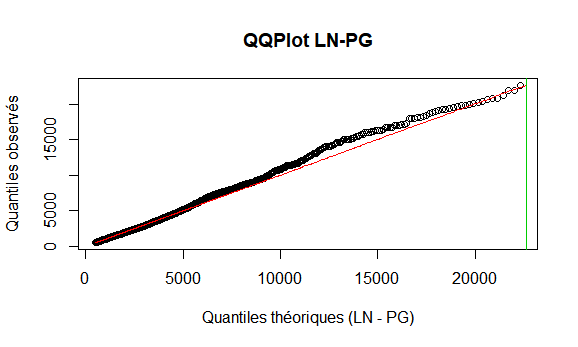
\includegraphics[scale=0.54]{Graphiques/QQ_LN_PG_choix_t1} 
					\caption{Quantiles de la lognormale pour $x<\theta$.} \label{QQplot_LN_PG_choix_2}
				\end{subfigure}
				\renewcommand{\figurename}{Illustration}
				\caption{\textit{QQplots} - \texttt{norwegianfire} - LN-PG - $\theta$ fixé.}
			\end{center}
		\end{figure}
		
		De nouveau, lorsqu'on regarde l'illustration \ref{QQplot_LN_PG_choix_2}, on voit que, lorsque l'on détermine un $\theta$ arbitrairement (sans tenir compte de la continuité et de la dérivabilité), on obtient une meilleure adéquation du modèle.
		
		\paragraph{Loi composite lognormale - Pareto - Pareto:} Les résultats obtenus avec la fonction \texttt{ConstrOptim} pour le cas où on a la continuité et la dérivabilité aux points $\theta_1$ et $\theta_2$ ne sont pas satisfaisants. Les résultats varient trop en fonction des paramètres initiaux fixés; particulièrement lorsque l'on fixe la valeur initiale de $\theta_1$ et de $\theta_2$.\\
	
		Si on applique la continuité et la dérivabilité seulement au point $\theta_1$, mais que l'on fixe $\theta_2 = 31\,728 $ on obtient $\hat{\theta_1} =1\,287,998\,125 $, $\hat{\alpha_1} =  1,282\,457$ et $\hat{\sigma}= 0,839\,466$, $\hat{\alpha_2}=1,458\,555$.
	
		\begin{figure}[H]
			\begin{center}
				\begin{subfigure}[b]{0.50\textwidth}
					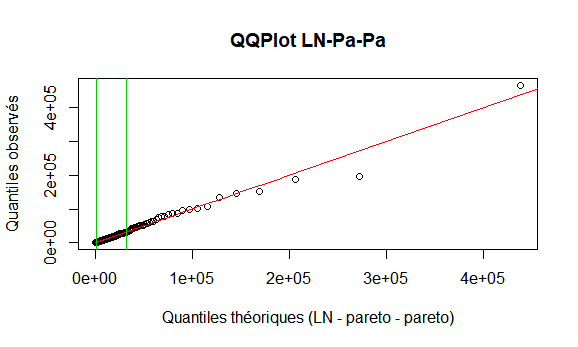
\includegraphics[scale=0.6]{Graphiques/QQ_LN_Pa_Pa_semi} 
					\caption{Quantiles sur le support complet.} \label{QQplot_LN_PaPa_semi}
				\end{subfigure}
				\begin{subfigure}[b]{0.42\textwidth}
					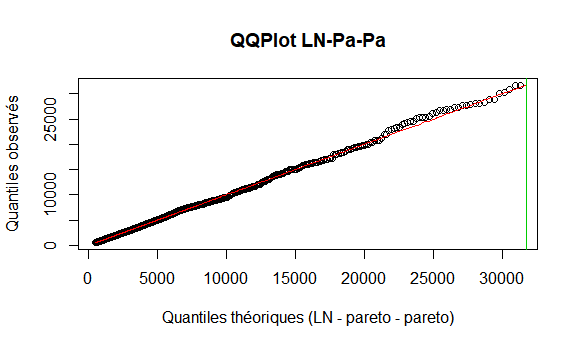
\includegraphics[scale=0.56]{Graphiques/QQ_LN_Pa_Pa_semi_t1} 
					\caption{Quantiles de la lognormale et $1^{ere}$ Pareto pour $x<\theta_2$.} \label{QQplot_LN_PaPa_semi_t1}
				\end{subfigure}
				\renewcommand{\figurename}{Illustration}
				\caption{\textit{QQplots} - \texttt{norwegianfire} - LN-Pa-Pa.}
			\end{center}
		\end{figure}
	
		Dans le illustration \ref{QQplot_LN_PaPa_semi}, on voit que les quantiles estimés sont comparables aux quantiles empiriques, même pour les valeurs très élevées.
		
		\paragraph{Loi composite Weibull et Pareto simple:} Avec la continuité et la dérivabilité au point $\theta$, on estime les paramètres et on obtient $\hat{\theta} = 1\,941,104\,864$, $\hat{\alpha} = 1,324\,505$ et $\hat{\tau}=0,595\,968$.
		
		\begin{figure}[H]
			\begin{center}
				\begin{subfigure}[b]{0.45\textwidth}
					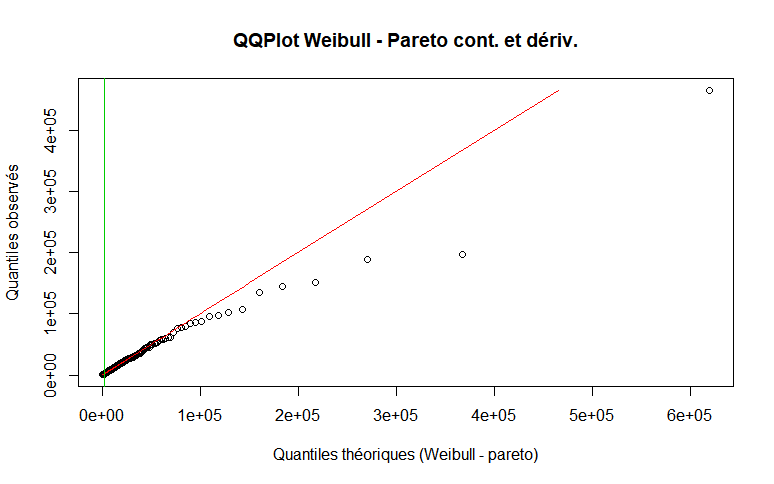
\includegraphics[scale=0.40]{Graphiques/QQ_Wei_Pa_contderiv} 
					\caption{Quantiles sur le support complet.} \label{QQplot_W_Pa_conde}
				\end{subfigure}
				\begin{subfigure}[b]{0.40\textwidth}
					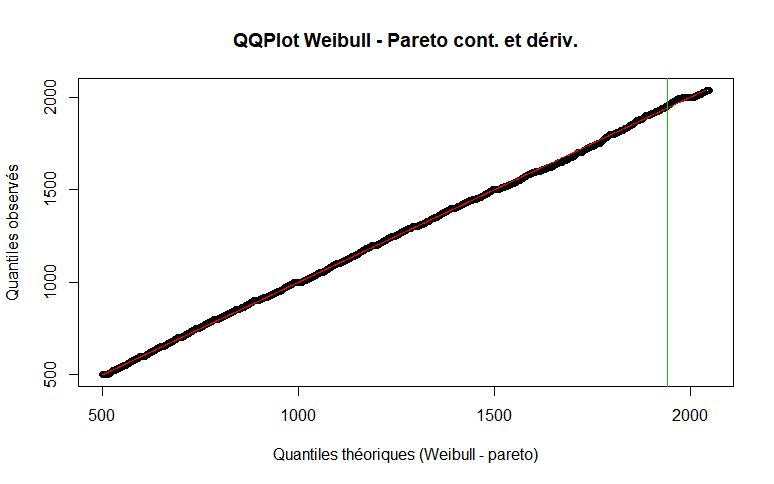
\includegraphics[scale=0.40]{Graphiques/QQ_Wei_Pa_contderiv_t1} 
					\caption{Quantiles de la Weibull pour $x<\theta$.} \label{QQplot_W_Pa_conde_2}
				\end{subfigure}
				\renewcommand{\figurename}{Illustration}
				\caption{\textit{QQplots} - \texttt{norwegianfire} - Weibull-Pareto.}
			\end{center}
		\end{figure}
		
		Le résultat est similaire à celui obtenu avec le modèle lognormal - Pareto. Cependant, le seuil $\hat{\theta}$ du modèle lognormal-Pareto est plus petit que celui du modèle Weibull-Pareto. Cela signifie que davantage de données sont attribuées à la partie Weibull. Si on fixe $\theta = 22\,669$, on obtient $\hat{\tau} =0,259\,762$, $\hat{\phi}=4,287\,200$ et $\hat{\alpha} = 1,540\,549$.
		
		\begin{figure}[H]
			\begin{center}
				\begin{subfigure}[b]{0.45\textwidth}
					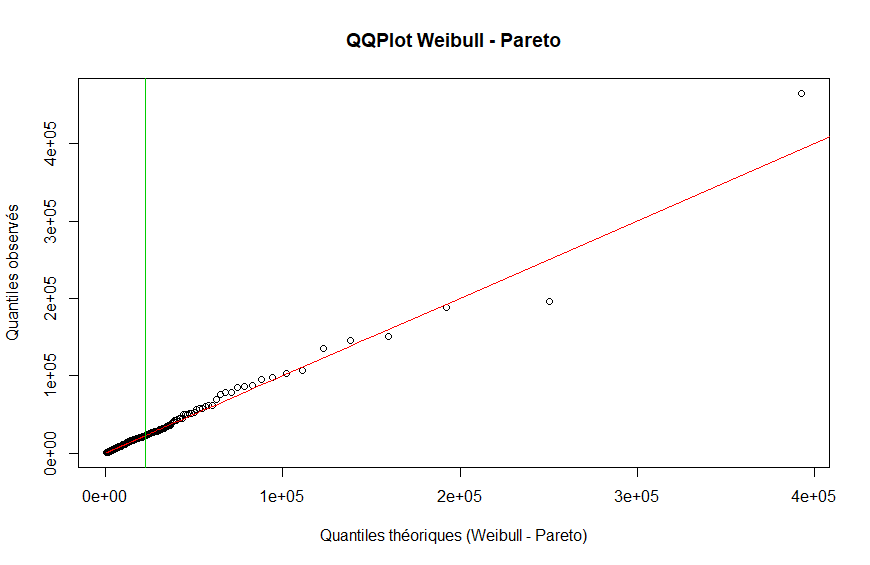
\includegraphics[scale=0.35]{Graphiques/QQ_Wei_pa_choix} 
					\caption{Quantiles sur le support complet.} \label{QQplot_Wei_pa_choix}
				\end{subfigure}
				\begin{subfigure}[b]{0.4\textwidth}
					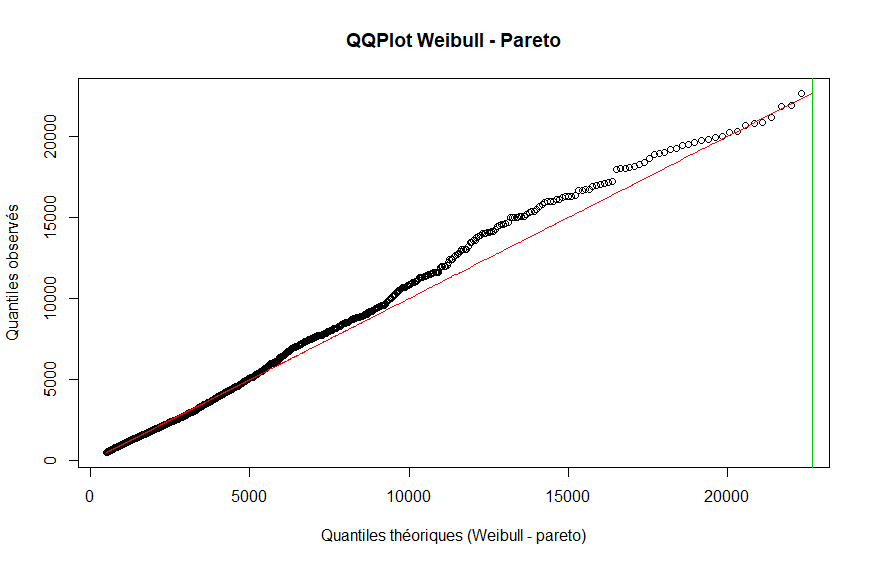
\includegraphics[scale=0.35]{Graphiques/QQ_Wei_pa_choix_t1} 
					\caption{Quantiles de la Weibull pour $x<\theta$.} \label{QQplot_Wei_pa_choix_2}
				\end{subfigure}
				\renewcommand{\figurename}{Illustration}
				\caption{\textit{QQplots} - \texttt{norwegianfire} - Weibull-Pareto - $\theta$ fixé.}\label{Wei_Pareto_Teta_fixe}
			\end{center}
		\end{figure}
	
		Dans l'illustration \ref{Wei_Pareto_Teta_fixe}, on voit que lorsque l'on fixe le seuil $\theta$, on peut obtenir une nette amélioration de l'adéquation des valeurs élevées, mais au prix d'une dégradation pour les petites valeurs.
		
		\paragraph{Loi composite Weibull et Pareto généralisée:} Avec la continuité et la dérivabilité au point $\theta$, on estime les paramètres et on obtient $\hat{\theta} = 1\,918,491\,146 $, $\hat{\alpha} = 1,327\,868 $ et $\hat{\tau}=0,599\,589 $ et $\hat{\lambda}=8,981\,391$.
		\begin{figure}[H]
			\begin{center}
				\begin{subfigure}[b]{0.45\textwidth}
					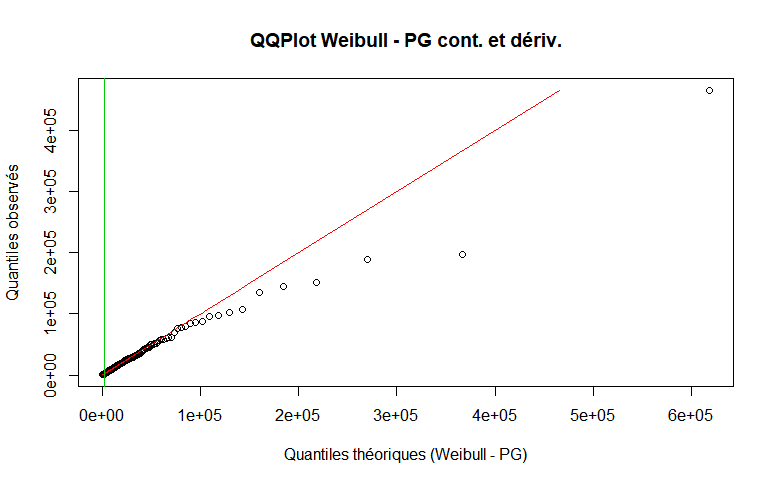
\includegraphics[scale=0.40]{Graphiques/QQ_Wei_PG_contderiv} 
					\caption{Quantiles sur le support complet.} \label{QQplot_W_PG_conde}
				\end{subfigure}
				\begin{subfigure}[b]{0.4\textwidth}
					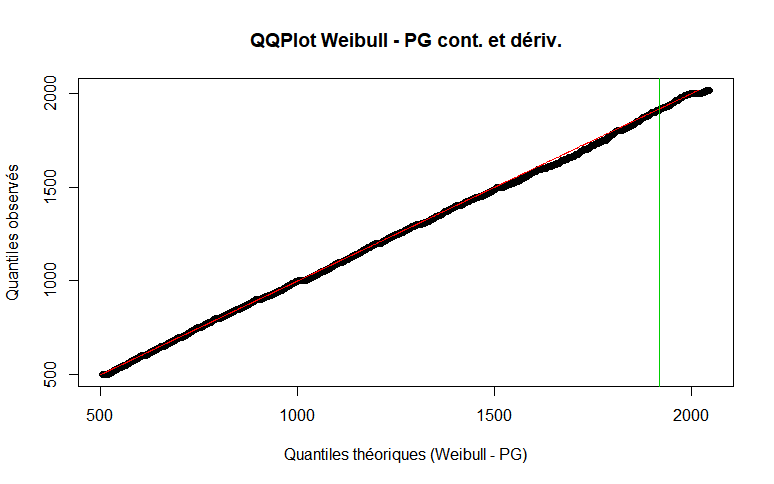
\includegraphics[scale=0.40]{Graphiques/QQ_Wei_PG_contderiv_t1} 
					\caption{Quantiles de la Weibull pour $x<\theta$.} \label{QQplot_W_PG_conde_2}
				\end{subfigure}
				\renewcommand{\figurename}{Illustration}
				\caption{\textit{QQplots} - \texttt{norwegianfire} - Weibull-PG.}
			\end{center}
		\end{figure}
		
		Les observations sont similaires à celles obtenues pour le modèle lognormal-Pareto et Weibull-Pareto.
		Si on fixe $\theta = 22\,669$, on obtient $\hat{\tau} =0,259\,762$, $\hat{\phi}=4,287\,198$, $\hat{\lambda}=4\,604,525\,53$ et $\hat{\alpha} = 1,728\,66$.
		
		\begin{figure}[H]
			\begin{center}
				\begin{subfigure}[b]{0.45\textwidth}
					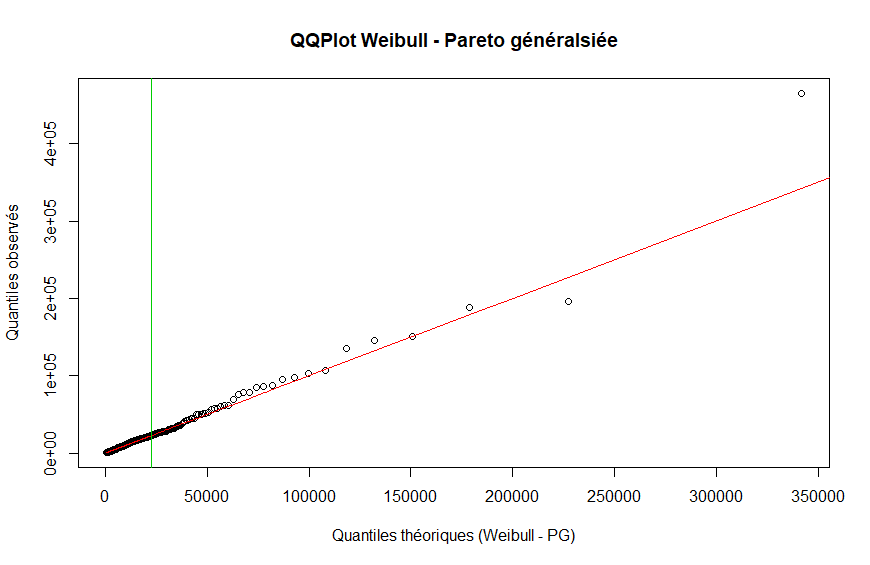
\includegraphics[scale=0.35]{Graphiques/QQ_Wei_PG_choix} 
					\caption{Quantiles sur le support complet.} \label{QQplot_Wei_PG_choix}
				\end{subfigure}
				\begin{subfigure}[b]{0.4\textwidth}
					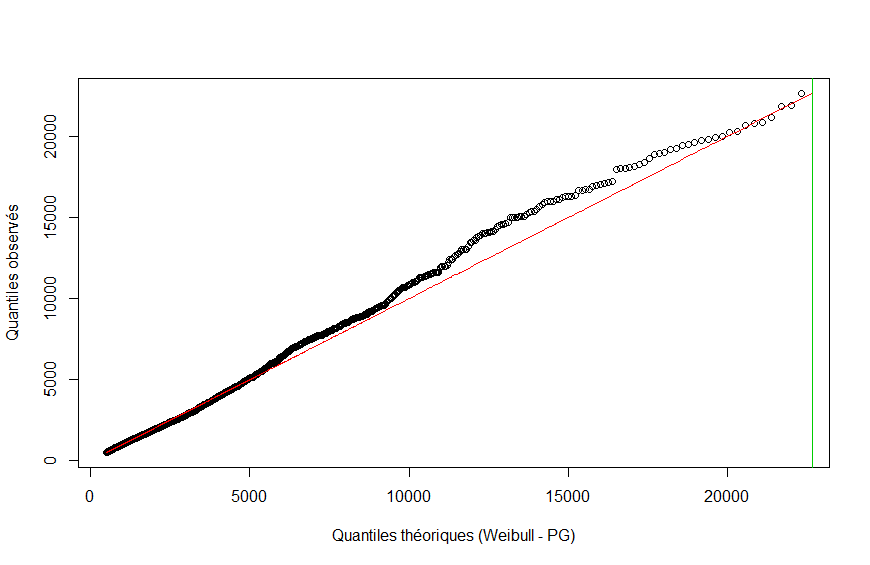
\includegraphics[scale=0.35]{Graphiques/QQ_Wei_PG_choix_t1} 
					\caption{Quantiles de la Weibull pour $x<\theta$.} \label{QQplot_Wei_PG_choix_2}
				\end{subfigure}
				\renewcommand{\figurename}{Illustration}
				\caption{\textit{QQplots} - \texttt{norwegianfire} - Weibull-Pareto - $\theta$ fixé.}\label{QQplot_Wei_PG_choix3}
			\end{center}
		\end{figure}
		À la lecture de l'illustration \ref{QQplot_Wei_PG_choix3}, on voit que les résultats sont très similaires à ceux obtenus avec les modèles utilisant une loi de Pareto simple pour représenter les grandes valeurs et dont le seuil $\theta$ est fixé.	
		
		\paragraph{Loi composite Weilbull - Pareto - Pareto:} Comme pour le modèle lognormal-Pareto-Pareto, les résultats obtenus en trouvant les deux seuils ($\theta_1$ et $\theta_2$) par optimisation numérique ne sont pas satisfaisants puisque la volatilité des paramètres obtenus est considérable. Pour cette raison, on fixe le deuxième seuil. Avec la continuité et la dérivabilité seulement au point $\theta_1$ et avec $\theta_2$ fixé à 31\,728, on obtient les paramètres $\hat{\theta_1} =1\,840,169\,474$, $\hat{\alpha_1} =  1,302\,509$ et $\hat{\tau}= 0,616\,114$, $\hat{\alpha_2}=1,458\,555$ 
		
		\begin{figure}[H]
			\begin{center}
				\begin{subfigure}[b]{0.45\textwidth}
					\includegraphics[scale=0.35]{Graphiques/QQ_Wei_Pa_Pa_semi} 
					\caption{Quantiles sur le support complet.} \label{QQplot_Wei_PaPa_semi}
				\end{subfigure}
				\begin{subfigure}[b]{0.4\textwidth}
					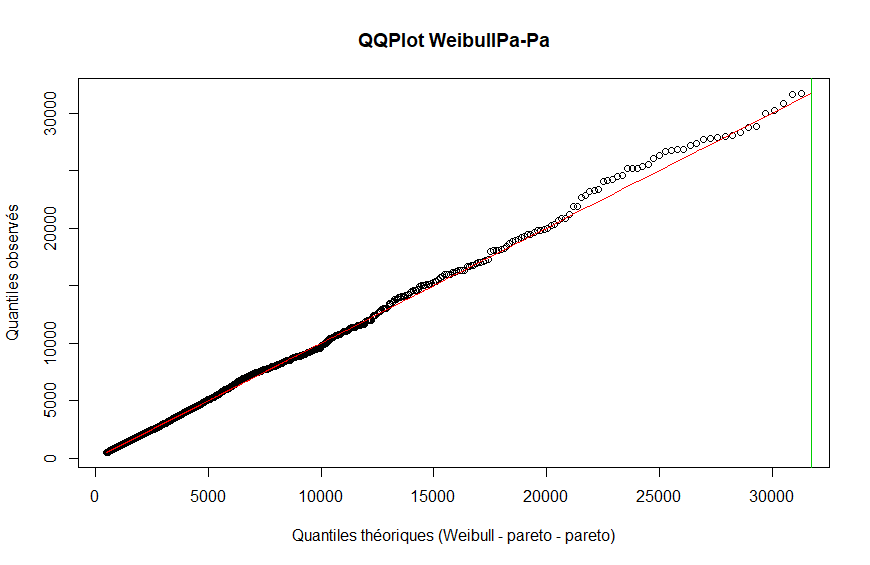
\includegraphics[scale=0.35]{Graphiques/QQ_Wei_Pa_Pa_semi_t1} 
					\caption{Quantiles de la Weibull pour $x<\theta$.} \label{QQplot_Wei_PaPa_semi_t1}
				\end{subfigure}
				\renewcommand{\figurename}{Illustration}
				\caption{\textit{QQplots} - \texttt{norwegianfire} - Weibull-Pa-Pa.}
			\end{center}
		\end{figure}
		
		\paragraph{Loi composite coxienne-2 - Pareto:} Avec la continuité au point $\theta$, on estime les paramètres et on obtient $\hat{\theta} =  6\,600,17$, $\hat{\alpha}= 1,347\,302$, $\hat{p} = 0,870\,677$, $\hat{\beta_1}=0,001\,940$ et $\hat{\beta_2}= 0,000\,427\,486$. Il faut noter que ces estimateurs ne sont pas optimaux puisqu'ils changent énormément selon les valeurs initiales choisies pour la fonction \texttt{ConstrOptim} de R. Cela peut être expliqué par le fait que la loi coxienne-2 possède trois paramètres. Si on considère que ce phénomène est similaire à celui obtenu avec les raccordements de trois lois, on peut conclure que la fonction d'optimisation numérique utilisée perd beaucoup de précision lorsqu'il y a plus de quatre paramètres à estimer.
		\begin{figure}[H]
			\begin{center}
				\begin{subfigure}[b]{0.45\textwidth}
					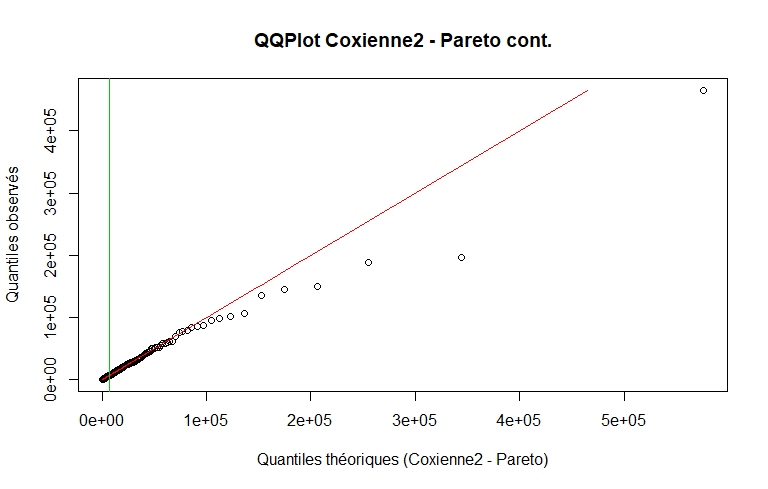
\includegraphics[scale=0.40]{Graphiques/QQ_Cox_Pa_cont} 
					\caption{Quantiles sur le support complet.} \label{QQplot_Cox_Pa_con}
				\end{subfigure}
				\begin{subfigure}[b]{0.4\textwidth}
					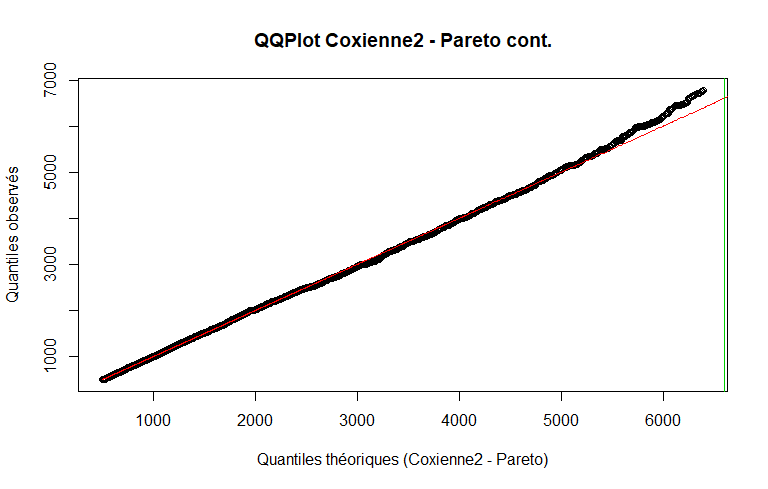
\includegraphics[scale=0.40]{Graphiques/QQ_Cox_Pa_cont_t1} 
					\caption{Quantiles de la cox-2 pour $x<\theta$.} \label{QQplot_Cox_Pa_con_2}
				\end{subfigure}
				\renewcommand{\figurename}{Illustration}
				\caption{\textit{QQplots} - \texttt{norwegianfire} - Coxienne-2 - Pareto.}\label{QQplot_Cox_Pa_con_3}
			\end{center}
		\end{figure}
		
		Même si les valeurs ne sont pas nécessairement optimales, on voit malgré tout dans l'illustration \ref{QQplot_Cox_Pa_con_3} que les valeurs inférieures à 100\,000 sont bien modélisés, mais que, pour les valeurs plus élevées, on obtient une surestimation des observations. \\
		
		Si on ignore la continuité, on fixe $\theta = 22\,669$ et on estime $\hat{\alpha} = 1,540\,549$, $\hat{p} =0,904\,056\,917$, $\hat{\beta_1}=0,001\,696\,942$ et $\hat{\beta_2} = 0,000\,262\,067$.
		
		\begin{figure}[H]
			\begin{center}
				\begin{subfigure}[b]{0.45\textwidth}
					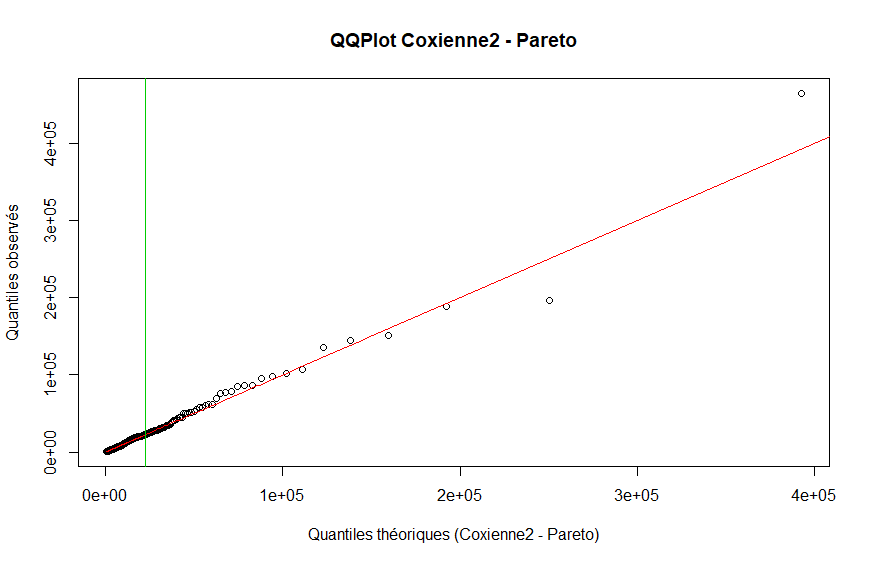
\includegraphics[scale=0.35]{Graphiques/QQ_Cox_pa_choix} 
					\caption{Quantiles sur le support complet.} \label{QQplot_Cox_pa_choix}
				\end{subfigure}
				\begin{subfigure}[b]{0.4\textwidth}
					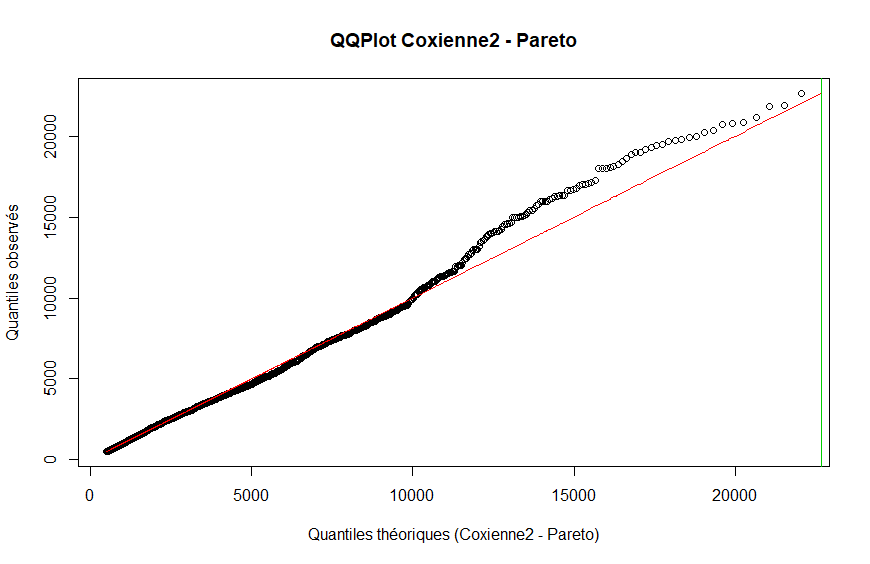
\includegraphics[scale=0.35]{Graphiques/QQ_Cox_pa_choix_t1} 
					\caption{Quantiles de la cox-2 pour $x<\theta$.} \label{QQplot_Cox_pa_choix_2}
				\end{subfigure}
				\renewcommand{\figurename}{Illustration}
				\caption{\textit{QQplots} - \texttt{norwegianfire} - Coxienne-2 - Pareto - $\theta$ fixé.}
			\end{center}
		\end{figure}
		L'ajustement est considérablement moins bon pour la partie coxienne-2, mais meilleur pour les valeurs très élevées.
		 
		\paragraph{Loi composite coxienne-2 - Pareto généralisée:} Avec la continuité au point $\theta$ on estime les paramètres et on obtient $\hat{\theta} =  7\,258,73$, $\hat{\lambda}=1\,057,91$, $\hat{\alpha}= 1,494\,710$ $\hat{p} = 0,561\,217$, $\hat{\beta_1}=0,001\,907\,145$ et $\hat{\beta_2}= 0,000\,408\,597$.
		
		\begin{figure}[H]
			\begin{center}
				\begin{subfigure}[b]{0.45\textwidth}
					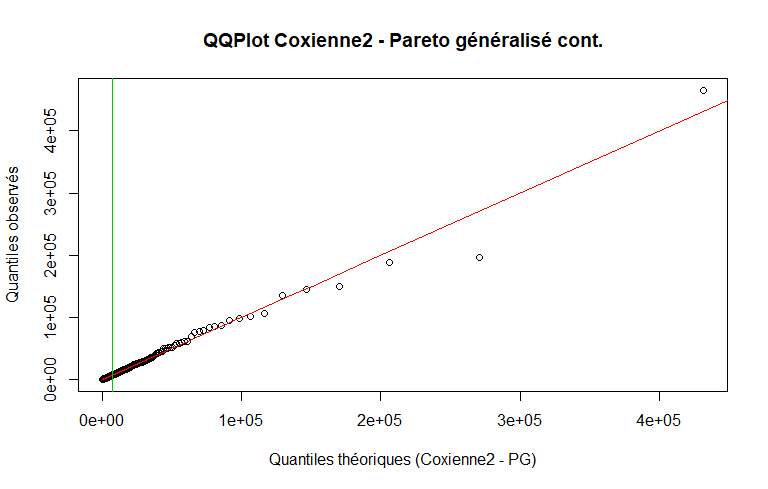
\includegraphics[scale=0.40]{Graphiques/QQ_Cox_PG_cont} 
					\caption{Quantiles sur le support complet.} \label{QQplot_Cox_PG_con}
				\end{subfigure}
				\begin{subfigure}[b]{0.4\textwidth}
					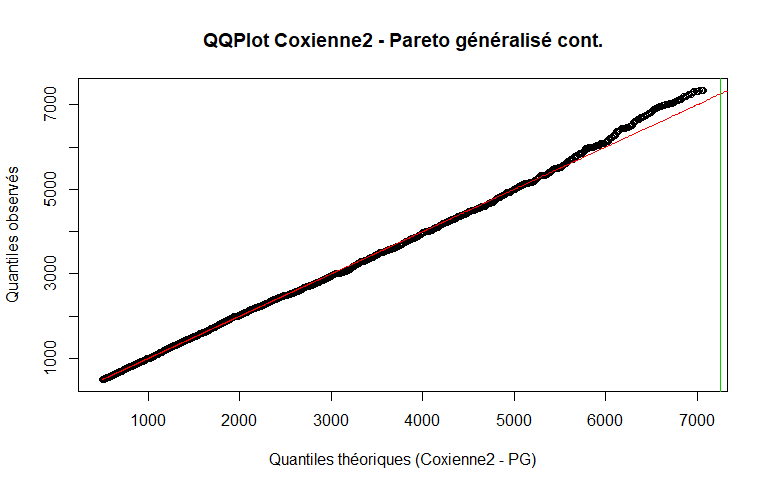
\includegraphics[scale=0.40]{Graphiques/QQ_Cox_PG_cont_t1} 
					\caption{Quantiles de la cox-2 pour $x<\theta$.} \label{QQplot_Cox_PG_con_2}
				\end{subfigure}
				\renewcommand{\figurename}{Illustration}
				\caption{\textit{QQplots} - \texttt{norwegianfire} - Coxienne-2 - PG. }
			\end{center}
		\end{figure}
		
		L'ajustement est acceptable pour les deux parties du raccordement. Si on ignore la continuité, on fixe $\theta = 22\,669$ et on estime $\hat{\lambda}=4\,604,525\,53$, $\hat{\alpha} = 1,728\,66$, $\hat{p} =0,904\,056\,917$, $\hat{\beta_1}=0,001\,696\,942$ et $\hat{\beta_2} = 0,000\,262\,067$.
		
		\begin{figure}[H]
			\begin{center}
				\begin{subfigure}[b]{0.45\textwidth}
					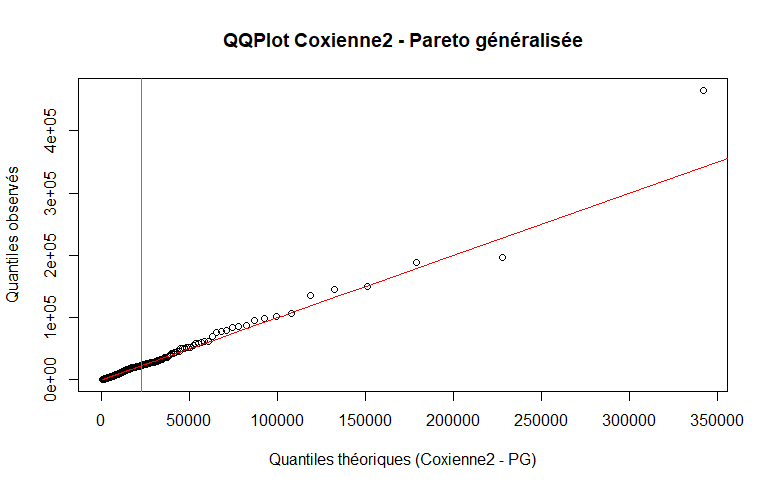
\includegraphics[scale=0.40]{Graphiques/QQ_Cox_PG_choix} 
					\caption{Quantiles sur le support complet.} \label{QQplot_Cox_PG_choix}
				\end{subfigure}
				\begin{subfigure}[b]{0.4\textwidth}
					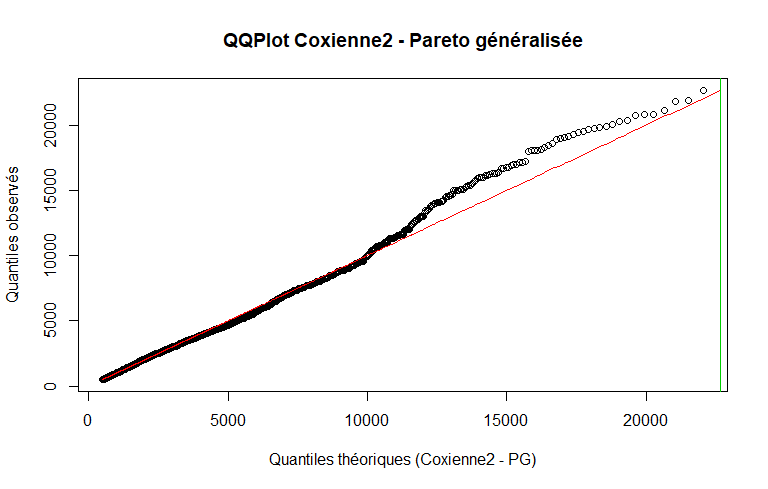
\includegraphics[scale=0.40]{Graphiques/QQ_Cox_PG_choix_t1} 
					\caption{Quantiles de la cox-2 pour $x<\theta$.} \label{QQplot_Cox_PG_choix_2}
				\end{subfigure}
				\renewcommand{\figurename}{Illustration}
				\caption{\textit{QQplots} - \texttt{norwegianfire} - Coxienne-2 - PG - $\theta$ fixé.}
			\end{center}
		\end{figure}
		L'ajustement est considérablement moins bon pour la partie coxienne-2, mais meilleur pour les valeurs élevées.
		 
	\subsubsection{\texttt{secura}}	
		
		\paragraph{Loi composite lognormale - Pareto:} Avec la continuité et la dérivabilité au point $\theta$ on estime les paramètres et on obtient $\hat{\theta} = 3,263\,838$, $\hat{\alpha} = 3,540\,522$, $\hat{\mu}=0,569\,56$  et $\hat{\sigma}=0,416\,216$.
		
		\begin{figure}[H]
			\begin{center}
				\begin{subfigure}[b]{0.45\textwidth}
					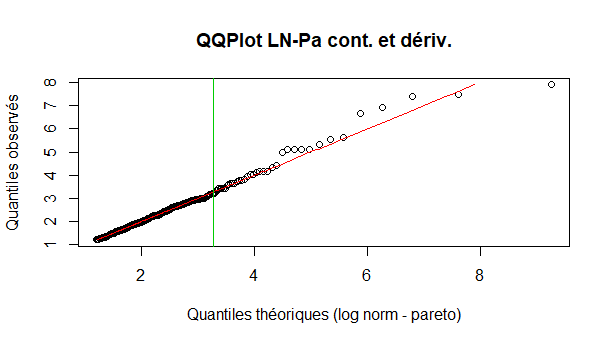
\includegraphics[scale=0.65]{Graphiques/QQ_LN_Pa_cont_dev_secura} 
					\caption{Quantiles sur le support complet.} \label{QQplot_LN_Pa_conde_sec}
				\end{subfigure}
				\begin{subfigure}[b]{0.4\textwidth}
					\includegraphics[scale=0.65]{Graphiques/QQ_LN_PA_contdiv_t1_secura} 
					\caption{Quantiles de la lognormale pour $x<\theta$.} \label{QQplot_LN_Pa_conde_2_sec}
				\end{subfigure}
				\renewcommand{\figurename}{Illustration}
				\caption{\textit{QQplots} - \texttt{secura} - Lognormale-Pareto.}
			\end{center}
		\end{figure}
		L'illustration \ref{QQplot_LN_Pa_conde_sec} montre un bon ajustement, même pour les valeurs élevées. Seulement les deux dernières statistiques d'ordre sont fortement surestimées. La portion lognormale comprend 62\% des données. \\
		
		Si on fixe le seuil, on regarde la fonction d'excès moyen présentée dans l'illustration \ref{Graph_Secura_MeanExcess} et on observe un changement de comportement à partir du point $3$. Conséquemment, on fixe $\theta = 3,001\,082$ et on estime $\hat{\mu} =0,574\,117$, $\hat{\sigma}=0,510\,611$ et $\hat{\alpha} = 3,279\,089$.
		
		\begin{figure}[H]
			\begin{center}
				\begin{subfigure}[b]{0.45\textwidth}
					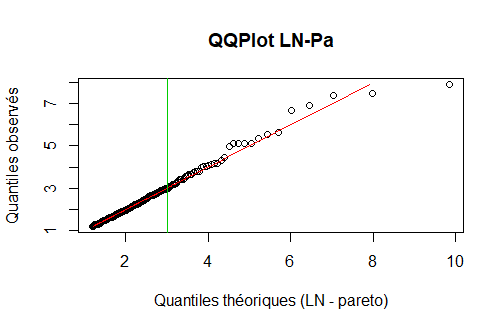
\includegraphics[scale=0.65]{Graphiques/QQ_LN_PA_choix_secura} 
					\caption{Quantiles sur le support complet.} \label{QQplot_LN_Pa_choix_secrua}
				\end{subfigure}
				\begin{subfigure}[b]{0.4\textwidth}
					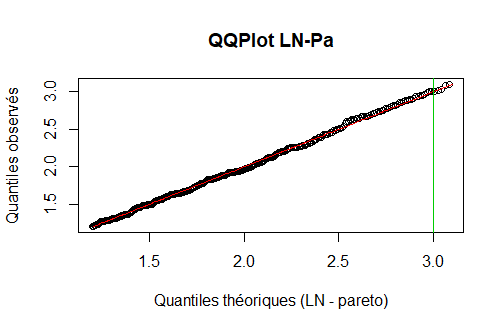
\includegraphics[scale=0.65]{Graphiques/QQ_LN_PA_choix_t1_secura} 
					\caption{Quantiles de la lognormale pour $x<\theta$.} \label{QQplot_LN_Pa_choix_2_secrua}
				\end{subfigure}
				\renewcommand{\figurename}{Illustration}
				\caption{\textit{QQplots} - \texttt{secura} - Lognormale-Pareto - $\theta$ fixé.}
			\end{center}
		\end{figure}
		
		L'ajustement est très similaire à celui présenté dans l'illustration \ref{QQplot_LN_Pa_conde_sec}, car on a fixe un $\theta$ proche de $\hat{\theta}$. Il est donc plus intéressant de choisir le modèle respectant les restrictions de continuité et de dérivabilité.  	

		\paragraph{Loi composite lognormale - Pareto généralisée:} Avec la continuité et la dérivabilité au point $\theta$ on estime les paramètres et on obtient $\hat{\theta} =3,150\,354$, $\hat{\lambda}=1,332\,734$ $\hat{\alpha} =4,896\,833 $ et $\hat{\sigma}= 0,418\,792$.
		\begin{figure}[H]
			\begin{center}
				\begin{subfigure}[b]{0.45\textwidth}
					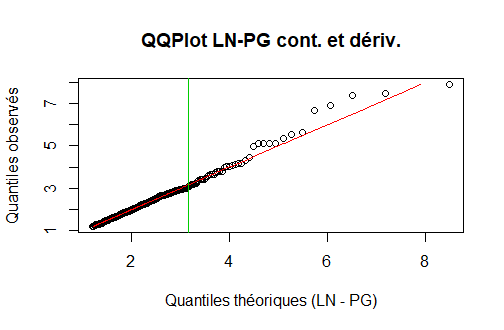
\includegraphics[scale=0.65]{Graphiques/QQ_LN_PG_condev_Secura} 
					\caption{Quantiles sur le support complet.} \label{QQplot_LN_PG_conde_Sec}
				\end{subfigure}
				\begin{subfigure}[b]{0.4\textwidth}
					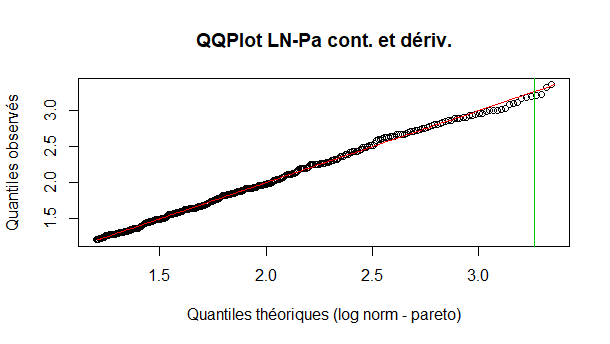
\includegraphics[scale=0.65]{Graphiques/QQ_LN_PA_contdiv_t1_Secura} 
					\caption{Quantiles de la lognormale pour $x<\theta$.} \label{QQplot_LN_PG_conde_2_Sec}
				\end{subfigure}
				\renewcommand{\figurename}{Illustration}
				\caption{\textit{QQplots} - \texttt{secura} - Lognormale-PG.}\label{QQplot_LN_PG_conde_Sec3}
			\end{center}
		\end{figure}
		
		Dans l'illustration \ref{QQplot_LN_PG_conde_Sec} on observe que le modèle avec une Pareto généralisée sous-estime davantage les grandes valeurs que le modèle avec une loi de Pareto simple. En revanche, la dernière valeur est beaucoup mieux prédite. La partie de la lognormale comprends 88\% des données, ce qui est plus élevé que lorsque l'on utilise la loi de Pareto simple pour modéliser les grandes valeurs. \\
		
		Si on ignore la continuité et la dérivabilité, on fixe $\theta = 3$ et on estime $\hat{\mu} =0,574\,117$, $\hat{\sigma}=0,510\,611$, $\hat{\lambda} =  23,788\,65$ et $\hat{\alpha} = 22,889\,47$. Il faut noter que $\hat{\alpha}$ est très grand pour une Pareto généralisée. Pour cette raison, la portion Pareto ressemble beaucoup à une loi gamma.
		
		\begin{figure}[H]
			\begin{center}
				\begin{subfigure}[b]{0.45\textwidth}
					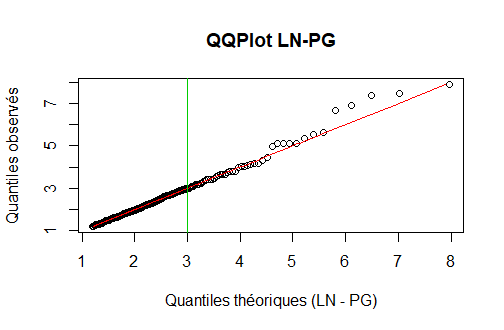
\includegraphics[scale=0.65]{Graphiques/QQ_LN_PG_choix_secura} 
					\caption{Quantiles sur le support complet.} \label{QQplot_LN_PG_choix_secura}
				\end{subfigure}
				\begin{subfigure}[b]{0.4\textwidth}
					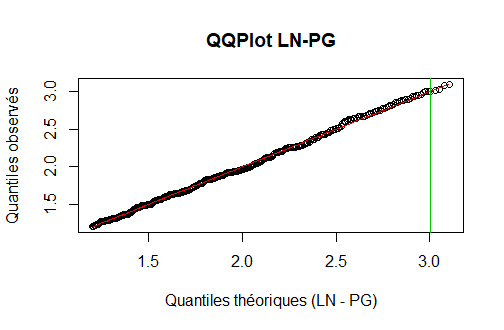
\includegraphics[scale=0.65]{Graphiques/QQ_LN_PG_choix_t1_secura} 
					\caption{Quantiles de la lognormale pour $x<\theta$.} \label{QQplot_LN_PG_choix_2_secura}
				\end{subfigure}
				\renewcommand{\figurename}{Illustration}
				\caption{\textit{QQplots} - \texttt{secura} - Lognormale-PG - $\theta$ fixé.}
			\end{center}
		\end{figure}
		Dans l'illustration \ref{QQplot_LN_PG_choix_secura}, on voit que l'adéquation globale lorsque l'on fixe le point $\theta$ est très similaire à celle lorsqu'on assume la continuité et la dérivabilité. Cependant, pour la plus grande valeur, celle-ci est mieux représentée lorsque le seuil est fixé.
		
		\paragraph{Loi composite lognormale - Pareto - Pareto:} Avec la continuité et la dérivabilité appliquée seulement au point $\theta_1$ et avec le point $\theta_2$ fixé à $4,050\,863$, on obtient $\hat{\theta_1} =2,247\,724 $, $\hat{\alpha_1} = 2,788\,940$, $\hat{\sigma}= 0,319\,746$ et $\hat{\alpha_2}=3,639\,318$.
		
		\begin{figure}[H]
			\begin{center}
				\begin{subfigure}[b]{0.45\textwidth}
					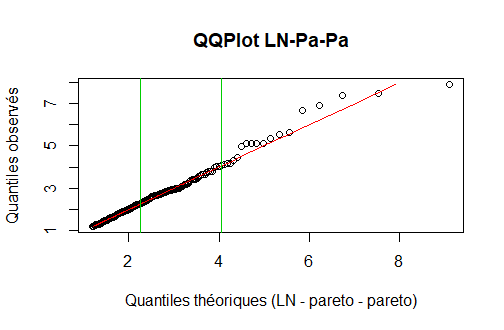
\includegraphics[scale=0.65]{Graphiques/QQ_LN_Pa_Pa_semi_Secura} 
					\caption{Quantiles sur le support complet.} \label{QQplot_LN_PaPa_semi_Sec}
				\end{subfigure}
				\begin{subfigure}[b]{0.4\textwidth}
					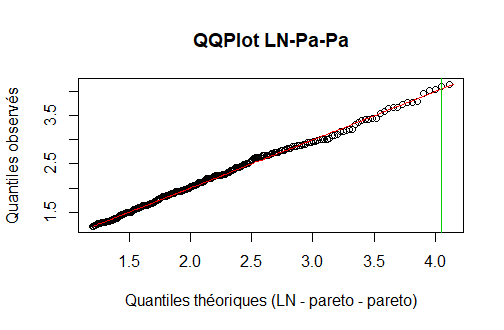
\includegraphics[scale=0.65]{Graphiques/QQ_LN_Pa_Pa_semi_t1_Secura} 
					\caption{Quantiles de la lognormale et $1^{ere}$ Pareto pour $x<\theta_2$.} \label{QQplot_LN_PaPa_semi_t1_sec}
				\end{subfigure}
				\renewcommand{\figurename}{Illustration}
				\caption{\textit{QQplots} - \texttt{secura} - Lognormale-Pa-Pa.}
			\end{center}
		\end{figure}
		Si on compare les illustrations \ref{QQplot_LN_PaPa_semi_Sec} et \ref{QQplot_LN_PG_conde_Sec}, on voit qu'il ne semble pas y avoir de réel avantage à utiliser un raccordement de trois lois pour modéliser les données. En effet, à première vue, il ne semble pas y avoir de différence significative pour les points se situant entre les deux seuils, de même que pour les valeurs élevées. 
		
		\paragraph{Loi composite Weibull - Pareto simple:} Avec la continuité et la dérivabilité au point $\theta$, on estime les paramètres et on obtient $\hat{\theta} = 2,992\,916$, $\hat{\alpha} = 3,571\,568$ et $\hat{\tau}= 2,034\,399$.
		\begin{figure}[H]
			\begin{center}
				\begin{subfigure}[b]{0.45\textwidth}
					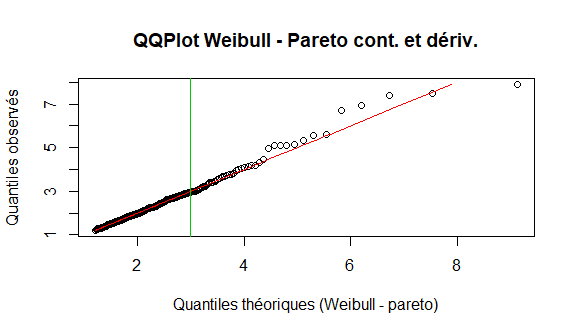
\includegraphics[scale=0.55]{Graphiques/QQ_Wei_Pa_contderiv_secura} 
					\caption{Quantiles sur le support complet.} \label{QQplot_W_Pa_conde_secura}
				\end{subfigure}
				\begin{subfigure}[b]{0.4\textwidth}
					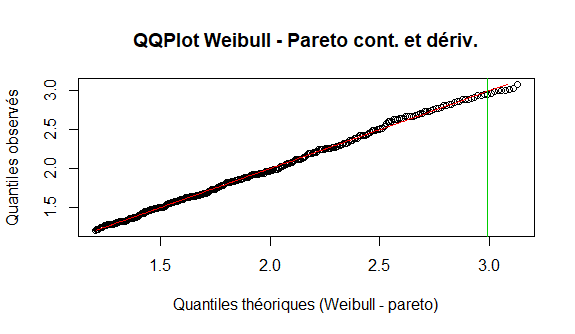
\includegraphics[scale=0.55]{Graphiques/QQ_Wei_Pa_contderiv_t1_secura} 
					\caption{Quantiles de la Weibull pour $x < \theta$.} \label{QQplot_W_Pa_conde_2_secura}
				\end{subfigure}
				\renewcommand{\figurename}{Illustration}
				\caption{\textit{QQplots} - \texttt{secura} - Weibull-Pareto.}
			\end{center}
		\end{figure}
		
		Visuellement, il est difficile d'identifier une différence entre ce modèle et le modèle lognormale. Par contre, le seuil $\theta$ est plus petit pour le modèle avec une loi lognormale que pour celui avec une loi Weibull. \\
		
		Si on fixe $\theta = 3$ et on estime $\hat{\tau} =1,718\,838$, $\hat{\phi}=1,811\,440$ et $\hat{\alpha} = 3,279\,089$.
		
		\begin{figure}[H]
			\begin{center}
				\begin{subfigure}[b]{0.45\textwidth}
					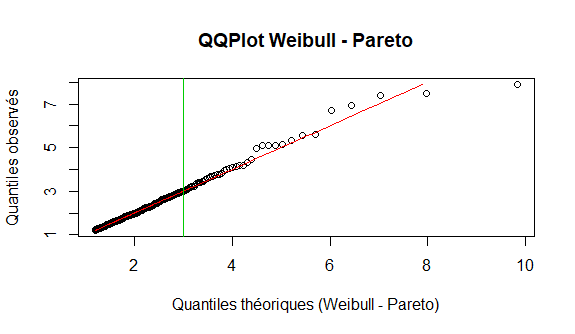
\includegraphics[scale=0.55]{Graphiques/QQ_Wei_pa_choix_secura} 
					\caption{Quantiles sur le support complet.} \label{QQplot_Wei_pa_choix_secura}
				\end{subfigure}
				\begin{subfigure}[b]{0.4\textwidth}
					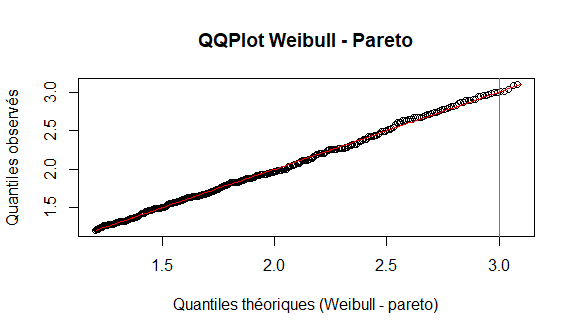
\includegraphics[scale=0.55]{Graphiques/QQ_Wei_pa_choix_t1_secura} 
					\caption{Quantiles de la Weibull pour $x < \theta$.} \label{QQplot_Wei_pa_choix_2_secura}
				\end{subfigure}
				\renewcommand{\figurename}{Illustration}
				\caption{\textit{QQplots} - \texttt{secura} - Weibull-Pareto - $\theta$ fixé.}
			\end{center}
		\end{figure}
	
		\paragraph{Loi composite Weibull - Pareto généralisée:} Avec la continuité et la dérivabilité au point $\theta$ on estime les paramètres et on obtient $\hat{\theta} = 2,944\,522 $, $\hat{\alpha} =  3,963\,976 $ et $\hat{\tau}=2,034\,156 $ et $\hat{\lambda}=0,372\,262$.
	
		\begin{figure}[H]
			\begin{center}
				\begin{subfigure}[b]{0.45\textwidth}
					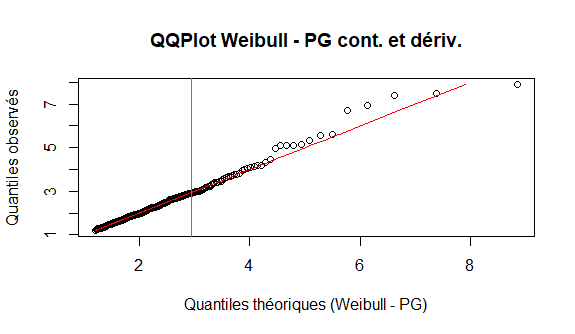
\includegraphics[scale=0.55]{Graphiques/QQ_Wei_PG_contderiv_secura} 
					\caption{Quantiles sur le support complet.} \label{QQplot_W_PG_conde_secura}
				\end{subfigure}
				\begin{subfigure}[b]{0.4\textwidth}
					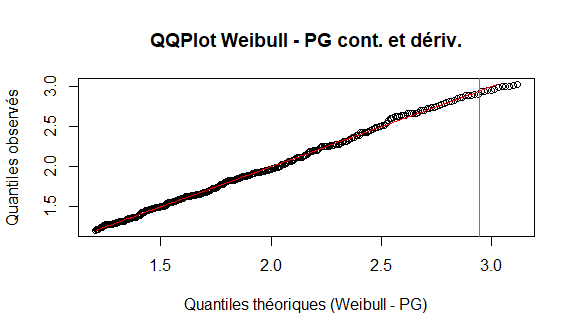
\includegraphics[scale=0.55]{Graphiques/QQ_Wei_PG_contderiv_t1_secura} 
					\caption{Quantiles de la Weibull pour $x < \theta$.} \label{QQplot_W_PG_conde_2_secura}
				\end{subfigure}
				\renewcommand{\figurename}{Illustration}
				\caption{\textit{QQplots} - \texttt{secura} - Weibull-PG.}
			\end{center}
		\end{figure}
		
		Si on fixe $\theta =3$, on obtient $\hat{\tau} =1,718\,838$, $\hat{\phi}=1,811\,440$, $\hat{\lambda}=23,788\,65$ et $\hat{\alpha} = 22,889\,47$.
		
		\begin{figure}[H]
			\begin{center}
				\begin{subfigure}[b]{0.45\textwidth}
					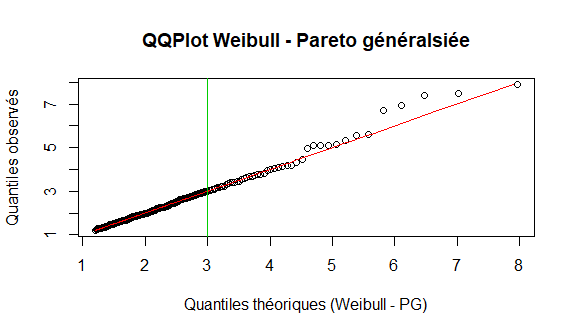
\includegraphics[scale=0.55]{Graphiques/QQ_Wei_PG_choix_secura} 
					\caption{Quantiles sur le support complet.} \label{QQplot_Wei_PG_choix_secura}
				\end{subfigure}
				\begin{subfigure}[b]{0.4\textwidth}
					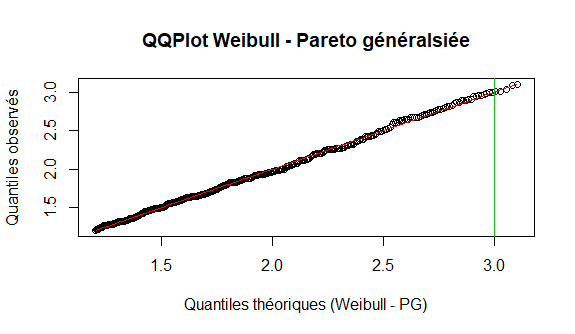
\includegraphics[scale=0.55]{Graphiques/QQ_Wei_PG_choix_t1_secura} 
					\caption{Quantiles de la Weibull pour $x < \theta$.} \label{QQplot_Wei_PG_choix_2_secura}
				\end{subfigure}
				\renewcommand{\figurename}{Illustration}
				\caption{\textit{QQplots} - \texttt{secura} - Weibull-PG - $\theta$ fixé.}
			\end{center}
		\end{figure}
		Mêmes observations que dans les section précédentes.
		
		\paragraph{Loi composite Weilbull - Pareto - Pareto:} Comme il a été conclu à la page \pageref{QQplot_Cox_Pa_con_3} les lois composites avec plus de quatre paramètres ont une forte volatilité. Malgré tout, si on assume la continuité et la dérivabilité seulement au point $\theta_1$ et qu'on fixe $\theta_2 = 4 $, on obtient $\hat{\theta_1} =3,060\,834$, $\hat{\alpha_1} =  3,886\,627$ et $\hat{\tau}= 2,054\,345$, $\hat{\alpha_2}=3,639\,318$. 
		
		\begin{figure}[H]
			\begin{center}
				\begin{subfigure}[b]{0.45\textwidth}
					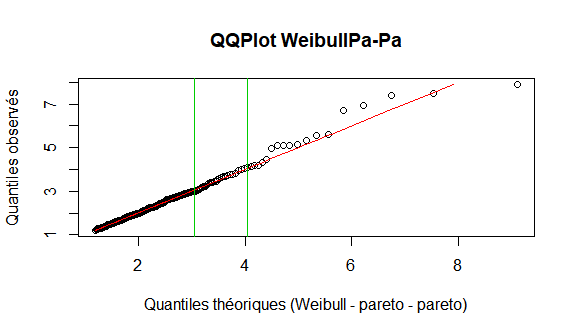
\includegraphics[scale=0.55]{Graphiques/QQ_Wei_Pa_Pa_semi_secura} 
					\caption{Quantiles sur le support complet.} \label{QQplot_Wei_PaPa_semi_secura}
				\end{subfigure}
				\begin{subfigure}[b]{0.4\textwidth}
					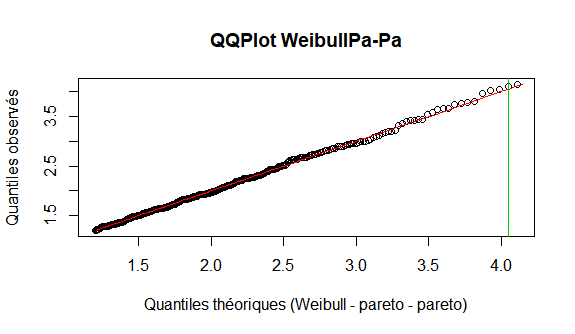
\includegraphics[scale=0.55]{Graphiques/QQ_Wei_Pa_Pa_semi_t1_secura} 
					\caption{Quantiles de la Weibull et $1^{ere}$ Pareto pour $x<\theta_2$.} \label{QQplot_Wei_PaPa_semi_t1_secura}
				\end{subfigure}
				\renewcommand{\figurename}{Illustration}
				\caption{\textit{QQplots} - \texttt{secura} - Weibull-Pa-Pa.}
			\end{center}
		\end{figure}
	
		\paragraph{Loi composite coxienne-2 - Pareto:} Avec la continuité au point $\theta$ on estime les paramètres et on obtient $\hat{\theta} = 2,274\,088$, $\hat{\alpha}= 3,236\,183$, $\hat{p} = 0,936\,706$, $\hat{\beta_1}=0,386\,105$ et $\hat{\beta_2}= 0,000\,012\,679$. Rappelons que ces valeurs ne sont pas optimales puisqu'elles varient beaucoup en fonction des valeurs initiales choisies pour la fonction \texttt{ConstrOptim} de R. 
		\begin{figure}[H]
			\begin{center}
				\begin{subfigure}[b]{0.45\textwidth}
					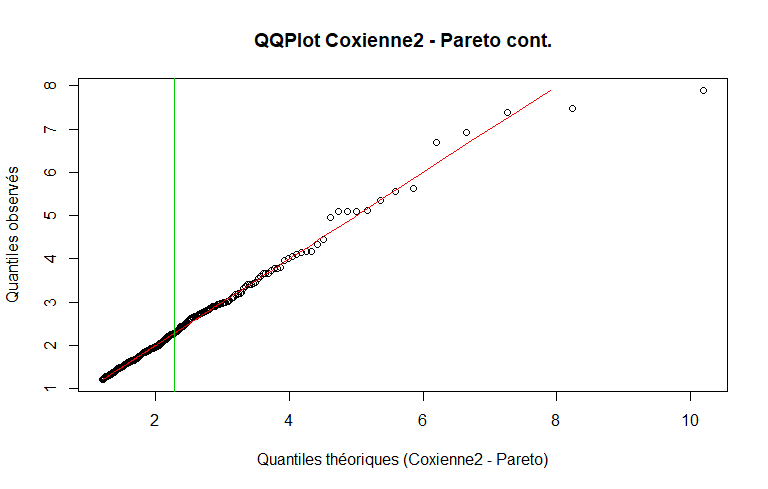
\includegraphics[scale=0.40]{Graphiques/QQ_Cox_Pa_cont_secura} 
					\caption{Quantiles sur le support complet.} \label{QQplot_Cox_Pa_con_sec}
				\end{subfigure}
				\begin{subfigure}[b]{0.4\textwidth}
					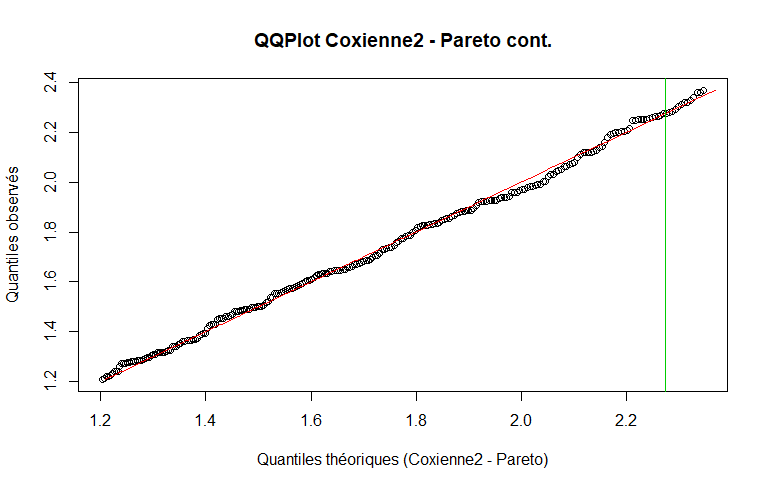
\includegraphics[scale=0.40]{Graphiques/QQ_Cox_Pa_cont_t1_secura} 
					\caption{Quantiles de la coxi-2 pour$ x<\theta$.} \label{QQplot_Cox_Pa_con_2_sec}
				\end{subfigure}
				\renewcommand{\figurename}{Illustration}
				\caption{\textit{QQplots} - \texttt{secura} - Coxienne-2 - Pareto.}
			\end{center}
		\end{figure}
		
		Même si les valeurs ne sont pas nécessairement optimales, l'illustration \ref{QQplot_Cox_Pa_con} nous montre un bon ajustement, sauf aux valeurs élevées.  \\
		
		Si on ignore la continuité, on fixe $\theta = 22\,669$ et on estime $\hat{\alpha} = 1,540\,549$, $\hat{p} =0,757\,712$, $\hat{\beta_1}=0,934\,538$ et $\hat{\beta_2} =0,000\,000\,013$.	
		\begin{figure}[H]
			\begin{center}
				\begin{subfigure}[b]{0.45\textwidth}
					\includegraphics[scale=0.40]{Graphiques/QQ_Cox_pa_choix_secura} 
					\caption{Quantiles sur le support complet.} \label{QQplot_Cox_pa_choix_sec}
				\end{subfigure}
				\begin{subfigure}[b]{0.4\textwidth}
					\includegraphics[scale=0.40]{Graphiques/QQ_Cox_pa_choix_t1_secura} 
					\caption{Quantiles de la cox-2 pour $x<\theta$.} \label{QQplot_Cox_pa_choix_2_sec}
				\end{subfigure}
				\renewcommand{\figurename}{Illustration}
				\caption{\textit{QQplots} - \texttt{secura} - Coxienne-2 - Pareto - $\theta$ fixé.}
			\end{center}
		\end{figure}
		L'ajustement est considérablement moins bon pour la partie coxienne-2, mais meilleur pour les valeurs élevées.\\
	
		\paragraph{Loi composite coxienne-2 - Pareto généralisée:} Avec la continuité au point $\theta$ on estime les paramètres et on obtient $\hat{\theta} =  2,669\,877$, $\hat{\lambda}=0,000\,005\,118$, $\hat{\alpha}= 3,695\,810$, $\hat{p} = 0,756\,522$, $\hat{\beta_1}=0,658\,269$ et $\hat{\beta_2}= 0,000\,000\,379\,863$. Encore ici, comme il y a six paramètres à estimer, il faut considérer la forte volatilité de ceux-ci.
		\begin{figure}[H]
			\begin{center}
				\begin{subfigure}[b]{0.45\textwidth}
					\includegraphics[scale=0.40]{Graphiques/QQ_Cox_PG_cont_secura} 
					\caption{Quantiles sur le support complet.} \label{QQplot_Cox_PG_con_sec}
				\end{subfigure}
				\begin{subfigure}[b]{0.4\textwidth}
					\includegraphics[scale=0.40]{Graphiques/QQ_Cox_PG_cont_t1_secura} 
					\caption{Quantiles de la cox-2 pour $x<\theta$.} \label{QQplot_Cox_PG_con_2_sec}
				\end{subfigure}
				\renewcommand{\figurename}{Illustration}
				\caption{\textit{QQplots} - \texttt{secura} - Coxienne-2 - PG.}
			\end{center}
		\end{figure}
	
	\subsubsection{\texttt{danish}}
		\paragraph{Loi de Pareto simple:}
		Comme il est mentionné dans la section \ref{Section_AnalysePreliminaire} et comme le confirme l'illustration \ref{QQplot_Par_t_Danish}, une simple loi de Pareto de type 1 fait un travail remarquable pour modéliser l'ensemble de la distribution de la base de données \texttt{danish}. Les paramètres de ce modèle sont $\hat{\lambda} =0,923\,065$ et $\hat{\alpha} =1,270\,676$.
		\begin{figure}[H]
			\centering
			\includegraphics[scale=0.70]{Graphiques/QQ_Pa_Danish}  
			\renewcommand{\figurename}{Illustration}
			\caption{\textit{QQplots} - \texttt{danish} - Pareto.} \label{QQplot_Par_t_Danish}
		\end{figure}

		Compte tenu qu'un modèle très simple réussit à donner d'aussi bons résultats, il est superflu de tester des modèles plus complexes qui ne risquent pas d'apporter d'amélioration significative.
			
	\subsection{Choix de modèle avec test d'adéquation}\label{Sect_Test_Adequation}
		Comme l'analyse graphique ne donne qu'un aperçu de l'adéquation des modèles, il est nécessaire de procéder à des tests statistiques pour compléter l'analyse des résultats et pour choisir un modèle propre à chacune des bases de données. À cet effet, on se base sur les trois tests suivants:
		\begin{enumerate}
			\item Anderson-Darling test
			\item AIC
			\item BSC
		\end{enumerate}  
		Comme le test Anderson-Darling est plus adéquat que le test Kolmogorov-Smirnov pour les distributions à queue lourde, il n'est pas nécessaire d'utiliser ce dernier. 
		
		\subsubsection{\texttt{norwegianfire}} 
		\begin{sloppypar}Le tableau \ref{TAB_TestGOF_NF} regroupe les résultats des trois tests pour chaque modèle de la base de données \texttt{norwegianfire}. Les modèles "$\theta$ fixé" désignent les modèles où on a choisit et fixé le point $\theta$ en ignorant la continuité et la dérivabilité. 
		\end{sloppypar}
		\begin{table}[H]
			\begin{center}
				\begin{tabular}{|l|cccc|}
					\hline
					Modèle sévérité          &         AIC         &         BSC         & A-D statistique & A-D valeur-p \\ \hline
					LN-Pa                    &     147\,702,2      &     147\,723,5      &       Inf       & 6,535236e-08 \\
					LN-Pa $\theta$ fixé      &     147\,733,7      &     147\,755,1      &       Inf       & 6,535236e-08 \\
					LN-PG                    &     147\,704,2      &     147\,732,7      &       Inf       & 6,535236e-08 \\
					LN-PG $\theta$ fixé      &     147\,733,6      &     147\,755,0      &       Inf       & 6,535236e-08 \\
					LN-Pa-Pa                 &     147\,706,4      &     147\,734,9      &       Inf       & 6,535236e-08 \\
					\textbf{Weibull-Pa }     & \textbf{147\,699,8} & \textbf{147\,721,2} & \textbf{89,225} & 6,535236e-08 \\
					Weibull-Pa $\theta$ fixé &     147\,746,2      &     147\,767,6      &       Inf       & 6,535236e-08 \\
					Weibull-PG               &     147\,701,8      &     147\,730,3      &       Inf       & 6,535236e-08 \\
					Weibull-Pa $\theta$ fixé &     147\,748,1      &     147\,776,6      &       Inf       & 6,535236e-08 \\
					Weibull-Pa-Pa            &     147\,700,4      &     147\,728,9      &       Inf       & 6,535236e-08 \\
					Cox2-Pa                  &     147\,721,7      &     147\,757,4      &   19\,781,082   & 6,535236e-08 \\
					Cox2-Pa $\theta$ fixé    &     147\,757,3      &     147\,785,8      &       Inf       & 6,535236e-08 \\
					Cox2-PG                  &     147\,725,8      &     147\,768,5      &   20\,747,655   & 6,535236e-08 \\
					Cox2-PG $\theta$ fixé    &     147\,759,1      &     147\,794,7      &       Inf       & 6,535236e-08 \\ \hline
				\end{tabular}
			\renewcommand{\tablename}{Tableau}
			\caption{Comparaison des modèles à l'aide les tests d'adéquation - \texttt{norwegianfire}.}\label{TAB_TestGOF_NF}
			\end{center}
		\end{table}
		La première chose que l'on observe est que, pour la majorité des modèles, la statistique d'Anderson-Darling retourne "Inf". Ceci est du à l'algorithme utilisé par la fonction \texttt{ad.test} du \textit{package} \texttt{Goftest}. En programmant directement \ref{Stat_AnedersonDarling2} dans \texttt{R}, on obtient des statistiques très grandes qui expliquent les résultats obtenus.	
		Or, ces valeurs élevées sont causées par le grand nombre d'observations (9181) de la base de données. Cela amplifie le poids accordé aux valeurs élevées. Comme on l'a vu avec l'analyse graphique, la majorité des modèles surestime les derniers quantiles. C'est pourquoi le test indique une mauvaise adéquation. La valeur-p, quant à elle, désigne la probabilité d'obtenir une statistique plus élevée. Comme les statistiques observées tendent déjà vers l'infini, la valeur-p tend vers zéro. \\
		
		Afin de choisir un modèle, lorsque l'on minimise l'AIC et le BSC, on trouve que le meilleur modèle est celui avec le raccordement des lois Weibull-Pareto simple. La statistique d'Anderson-Darling vient corroborer cette affirmation puisqu'il s'agit du modèle avec la statistique la plus faible. On obtient donc les paramètres $\hat{\theta}=1\,941,104\,864$, $\hat{\alpha}=1,324\,506$, $\hat{\tau}=0,595\,968$ et $\hat{\phi} = 272,486$.
		
		\subsubsection{\texttt{secura}} Du côté de \texttt{secura}, les résultats sont présentés dans le tableau \ref{TAB_TestGOF_Secura}. 
		\begin{table}[H]
		\centering
			\begin{tabular}{|l|cccc|}
				\hline			
				Modèle sévérité          &        AIC        &        BSC        &   A-D statistique    &     A-D valeur-p     \\ \hline
				LN-Pa                    &     757,7265      &     769,4751      &     0,193\,0576      &     0,992\,1934      \\
				LN-Pa $\theta$ fixé      &     755,4610      &     767,2097      &     0,211\,9562      &     0,986\,7947      \\
				LN-PG                    &     759,5169      &     775,1817      & \textbf{0,197\,9434} & \textbf{0,990\,9668} \\
				LN-PG $\theta$ fixé      & \textbf{753,9616} & \textbf{765,7102} &     0,210\,9490      &     0,987\,1276      \\
				LN-Pa-Pa                 &     758,6773      &     774,3421      &     0,354\,8336      &     0,891\,9703      \\
				Weibull-Pa               &     757,7968      &     769,5454      &     0,214\,5025      &     0,985\,9295      \\
				Weibull-Pa $\theta$ fixé &     756,1329      &     767,8815      &     0,262\,5257      &     0,963\,3705      \\
				Weibull-PG               &     759,7639      &     775,4287      &     0,217\,4760      &     0,984\,8769      \\
				Weibull-Pa $\theta$ fixé &     756,6335      &     772,2983      &     0,261\,5185      &     0,963\,9622      \\
				Weibull-Pa-Pa            &     759,6633      &     775,3281      &     0,209\,7732      &     0,987\,5097      \\
				Cox2-Pa                  &     764,6622      &     784,2433      &     0,338\,4047      &     0,906\,7163      \\
				Cox2-Pa $\theta$ fixé    &     770,8757      &     786,5405      &     1,920\,5081      &     0,101\,6452      \\
				Cox2-PG                  &     765,9469      &     789,4441      &     0,549\,5856      &     0,696\,7520      \\
				Cox2-PG $\theta$ fixé    &     771,2971      &     790,8781      &     1,916\,3475      &     0,102\,1868      \\ \hline
			\end{tabular}
			\renewcommand{\tablename}{Tableau}
			\caption{Comparaison des modèles à l'aide les testes d'adéquation - \texttt{secura}.}\label{TAB_TestGOF_Secura}
		\end{table}
	
		Contrairement à la base de données \texttt{norwegianfire}, pour \texttt{secura}, le test Anderson-Darling donne des statistiques près de zéro avec des valeurs-p qui sont près de un; cela signifie que les modèles sont adéquats. Mentionnons que cette base de données ne contient que 371 observations comparativement à son homologue qui en a 9\,181. \\

		Les valeurs de l'AIC et du BSC montrent que les modèles lognormal-Pareto simple et lognormal-Pareto généralisé, avec le seuil $\theta$ fixé, sont les plus convenables. Avec le test du ratio de vraisemblance, on rejette le modèle plus complexe en faveur de celui utilisant la loi composite lognormale-Pareto simple avec les paramètres $\hat{\theta}=3,263\,838$, $\hat{\alpha}=3,5205$, $\hat{\mu} = 0,56956$ et $\hat{\sigma}=0,416\,216$.\\
		
		Avec une valeur-p de 98,7\%, on a que le modèle lognormal-Pareto simple avec $\theta$ fixé possède une excellente adéquation.

	\subsection{Agrégation des modèles choisis}
	
		\subsubsection{\texttt{norwegianfire}}
		Pour modélisé la sévérité, comme il est expliqué dans la section \ref{Sect_Test_Adequation}, on a $X \sim Weibull\text{-}Pareto (\hat{\theta}=1\,941,104\,864,\: \hat{\alpha}=1,324\,506,\: \hat{\tau}=0,595\,968,\: \hat{\phi} = 272,486)$.\\
		
		Dans la section \ref{Section_AnalysePreliminaire}, on conclut que la fréquence est modélisée avec un processus de Poisson homogène ajusté sur les 3 dernières années; i.e. avec une intensité annuelle $\lambda$ de 622 sinistres par année.\\
		
		L'espérance conditionnelle de la Weibull-Pareto est de $E[X|X>500]=2\,529,774$. L'espérance de $S(t)$ est donc $E[S(t)]=E[N(t)]E[X]=1\,573\,519$. On utilise la méthode Monte Carlo afin d'obtenir les mesures de risques du modèle. Avec $100\,000$ simulations, on obtient $\widehat{E[S(t)|X>500]}=1\,547\,359$ qui est proche de l'espérance théorique.\\
		
		Le tableau \ref{TAB_TVAR_NF} fournit les mesures VaR et TVaR pour un $\kappa$ donné. Afin mieux comprendre les valeurs, on les compare avec les coûts totaux observés dans le tableau \ref{TAB_COUT_OBS_NF}.
		
		\begin{table}[H]
			\begin{center}
				\begin{tabular}{|c|c|c|}
					\hline
					$\kappa$ & $\widehat{VaR_{\kappa}}(S(t))$ & $\widehat{TVaR_{\kappa}}(S(t))$ \\ \hline
					0,9000   &         1\,871\,739         &         3\,086\,597          \\
					0,9500   &         2\,224\,579         &         4\,158\,473          \\
					0,9900   &         4\,053\,983         &         9\,822\,640          \\
					0,9990   &        14\,803\,941         &         40\,749\,977         \\
					0,9999   &        81\,907\,085         &        138\,464\,457         \\ \hline
				\end{tabular}
				\renewcommand{\tablename}{Tableau}
				\caption{VaR et TVaR avec 100\,000 simulations - \texttt{norwegianfire}.}\label{TAB_TVAR_NF}
			\end{center}
		\end{table}
		
		\begin{table}[H]
			\centering
				\begin{tabular}{|c|r|}
					\hline
					Année & Coûts totaux \\ \hline
					 72   &     184\,119 \\
					 73   &     211\,204 \\
					 74   &     226\,680 \\
					 75   &     286\,551 \\
					 76   &     574\,559 \\
					 77   &     520\,717 \\
					 78   &     605\,548 \\
					 79   &     601\,505 \\
					 80   &     642\,344 \\
					 81   &  1\,027\,037 \\
					 82   &     778\,403 \\
					 83   &     778\,796 \\
					 84   &  1\,120\,877 \\
					 85   &  1\,549\,490 \\
					 86   &  1\,602\,327 \\
					 87   &  1\,577\,655 \\
					 88   &  2\,626\,675 \\
					 89   &  1\,723\,077 \\
					 90   &  1\,239\,369 \\
					 91   &  1\,135\,961 \\
					 92   &  1\,343\,306 \\ \hline
				\end{tabular}
				\renewcommand{\tablename}{Tableau}
				\caption{Coûts totaux observés par année - \texttt{norwegianfire}.}\label{TAB_COUT_OBS_NF}
		\end{table}
	
		\begin{sloppypar} On observe que les $\widehat{TVaR_{\kappa}(S(t))}$ augmentent très rapidement avec $\kappa$. Ceci est dû au paramètre $\hat{\alpha}$ de la loi de Pareto qui est très près de 1. Déjà la $\widehat{TVaR_{0,9}}(S(t))$ est considérable et aucune année observée n'excède cette valeur. Comme il est démontré dans l'illustration \ref{QQplot_W_Pa_conde}, on surestime les valeurs élevées. De plus, la loi de fréquence choisie est basée seulement sur les 3 dernières années qui sont plus élevées que le reste des observations. Ces deux constats font en sorte que la $\widehat{TVaR_{\kappa}(S(t))}$ est probablement surestimée aussi. Pour cette raison, advenant qu'une compagnie d'assurance couvrirait ces données, il serait raisonnable de prendre un niveau de confiance de 90\% plutôt que 95\% ou 99\% pour mesurer le risque du portefeuille et, éventuellement, calculer le capital d'assurance.
		\end{sloppypar}	
	
		\subsubsection{\texttt{secura}}	
		Pour la base de données \texttt{secura}, on a $X \sim lognormale\text{-}Pareto(\hat{\theta}=3,263\,838,\:\hat{\alpha}=3,5205,\:\mu = 0,56956,\:\hat{\sigma}=0,416\,216)$ pour modéliser les montants de sinistres. Puis, la fréquence est modélisée par un processus de Poisson non homogène cyclique avec $\hat{a}=25,59688$, $\hat{b}=29,99606$ et $\hat{c}=15,04107$ dont la fonction de masse de probabilités pour une année donnée est 
		$$
		P[N(t+1)-N(t) =x ] = \frac{ \left(  a-\frac{bc}{2\pi}\left[\sin\left(\frac{2\pi(t+1)}{c}\right)-\sin\left(\frac{2\pi(t)}{c}\right)\right]  \right)^{x} e^{-\left(a-\frac{bc}{2\pi}\left[\sin\left(\frac{2\pi(t+1)}{c}\right)-\sin\left(\frac{2\pi(t)}{c}\right)\right] \right)} }{x}.
		$$
		
		Dans ce contexte, $c$ indique un cycle sur 15 ans. Cependant, comme il est mentionné dans la section \ref{Section_AnalysePreliminaire}, cet effet cyclique ne semble pas, \textit{a priori}, logique et devrait être valider pour tirer des conclusions formelles. \\
		
		L'espérance conditionnelle de la loi composite lognormale-Pareto est $E[X|X>1,2] =2,23676$. L'espérance du coût total annuel est de $E[S(t)|X>1,2]=30,16341$. En utilisant la méthode Monte Carlo, on obtient $\widehat{E[S(t)|X>1,2]}=30,14298$; ce qui est très près de la valeur théorique. Le tableau \ref{TAB_TVAR_Sec} présente les mesures VaR et TVaR pour un $\kappa$ donnée. Afin d'avoir un point de comparaison, on présente les montants totaux observés dans le tableau \ref{TAB_COUT_OBS_Sec}.
		
		\begin{table}[H]
			\begin{center}
				\begin{tabular}{|c|c|c|}
					\hline
					$\kappa$ & $\widehat{VaR_{\kappa}}(S(t))$ & $\widehat{TVaR_{\kappa}}(S(t))$ \\ \hline
					0,9000   &          42,20867           &           47,73302           \\
					0,9500   &          46,30457           &           51,40434           \\
					0,9900   &          54,39311           &           59,56204           \\
					0,9990   &          66,13426           &           74,10636           \\
					0,9999   &          78,07877           &          109,59834           \\ \hline
				\end{tabular}
				\renewcommand{\tablename}{Tableau}
				\caption{VaR et TVaR avec 100\,000 simulations - \texttt{secura}.}\label{TAB_TVAR_Sec}
			\end{center}
		\end{table}
	
		\begin{table}[H]
			\begin{center}
				\begin{tabular}{|l|c|}
					\hline
					Année & Coûts totaux (en millions) \\ \hline
					1988  &          34,89522          \\
					1989  &          31,59057          \\
					1990  &          48,06152          \\
					1991  &          88,28169          \\
					1992  &          65,26679          \\
					1993  &          64,41851          \\
					1994  &          44,49027          \\
					1995  &          83,39058          \\
					1996  &          84,95461          \\
					1997  &          81,84038          \\
					1998  &          68,39825          \\
					1999  &          56,19868          \\
					2000  &          60,49544          \\
					2001  &          15,29495          \\ \hline
				\end{tabular}
				\renewcommand{\tablename}{Tableau}
				\caption{Coûts totaux observés par année - \texttt{secura}.}\label{TAB_COUT_OBS_Sec}
			\end{center}
		\end{table}
	
		À la lecture du tableau \ref{TAB_TVAR_Sec}, on voit que les valeurs de la  $\widehat{TVaR_{\kappa}}(S(t))$ augmentent moins vite que pour celles obtenues avec \texttt{norwegianfire} étant donné que le paramètre de forme ($\alpha$) de la loi de Pareto est plus grand pour \texttt{secura} que pour \texttt{norwegianfire}. Un autre aspect qu'il faut observer lorsque l'on compare les tableaux \ref{TAB_TVAR_Sec} et \ref{TAB_COUT_OBS_Sec}, c'est qu'il y a trois années qui sont supérieures à la $\widehat{TVaR_{0,999}}(S(t))$. Une compagnie d'assurance qui couvrirait ce portefeuille devrait donc considérer un niveau de confiance d'au moins 99,99\% dans l'évaluation de ses réserves pour se protéger contre d'éventuelles pertes. Finalement, lorsque l'on observe l'année 2001, on voit que le montant total des sinistres est significativement plus faible que pour les autres années. Comme cette valeur est aberrante, il faudrait vérifier la raison de cet écart pour valider s'il faut l'ignorer, l'ajuster ou la considérer comme tel.
		
		\subsubsection{\texttt{danish}}
		Pour la base de données \texttt{danish}, on a $X \sim Pareto(\hat{\alpha} = 1,635\,637,\: \hat{\theta}=0,524\,450)$ et $N(t) \sim Poisson(\Lambda(t))$ avec intensité $\lambda(t) = 0,4283298 + 0,00005452899 t$. Le tableau \ref{TAB_TVAR_Dan} donne les VaR et TVaR estimées avec la méthode Monte Carlo.
		
		\begin{table}[H]
			\begin{center}
				\begin{tabular}{|c|c|c|}
					\hline
					$\kappa$ & $\widehat{VaR_{\kappa}}(S(t))$ & $\widehat{TVaR_{\kappa}}(S(t))$ \\ \hline
					0,9000   &           998,025           &          1\,363,013          \\
					0,9500   &         1\,129,939          &          1\,671,996          \\
					0,9900   &         1\,661,365          &          3\,197,928          \\
					0,9990   &         4\,370,091          &         11\,574,773          \\
					0,9999   &         19\,405,328         &         51\,744,558          \\ \hline
				\end{tabular}
				\renewcommand{\tablename}{Tableau}
				\caption{VaR et TVaR avec 100\,000 simulations - \texttt{danish}.}\label{TAB_TVAR_Dan}	
			\end{center}
		\end{table}
	
		\begin{table}[H]
			\begin{center}
				\begin{tabular}{|l|c|}
					\hline
					Année & Coûts totaux (en millions) \\ \hline
					1980  &          869,7132          \\
					1981  &          626,5116          \\
					1982  &          599,3166          \\
					1983  &          400,3404          \\
					1984  &          436,7605          \\
					1985  &          658,9297          \\
					1986  &          609,2502          \\
					1987  &          678,1011          \\
					1988  &          793,9485          \\
					1989  &          904,2201          \\
					1990  &          758,3944          \\ \hline
				\end{tabular}
				\renewcommand{\tablename}{Tableau}
				\caption{Coûts totaux observés par année - \texttt{danish}.}\label{TAB_COUT_OBS_Dan}	
			\end{center}
		\end{table}
	
		La $\widehat{TVaR_{\kappa}}(S(t))$ augmente fortement avec $\kappa$ étant donné le paramètre de forme ($\alpha$) qui tend vers 1. Cette distribution a donc une queue très lourde. De plus, on a une intensité qui augmente linéairement avec le temps, on s'attends donc à une augmentation de la fréquence des sinistres dans le future. Ce qui contribuera à une augmentation de la TVaR au fil du temps.   \\
		
		On voit également, lorsque l'on regarde le tableau \ref{TAB_COUT_OBS_Dan}, que, sur dix ans, aucune valeur n'a dépassé un million. Un niveau de confiance de 95\% ou 99\% pourrait donc, \textit{a priori}, être raisonnable pour calculer le montant des réserves.